%Empieza configuracion de capitulo
\setstretch{1.0}
\titleformat{\chapter}[block]{\Large\bfseries}{CAP'ITULO \Huge\thechapter\vspace{25 pt}}{0 pt}{\\\fontsize{26}{36}\selectfont}
\titlespacing{\chapter}{0 pt}{30 pt}{50 pt}[0 pt]
\titleformat{\section}{\Large\bfseries}{\thesection}{0 pt}{\hspace{30 pt}}
\titleformat{\subsection}{\large\bfseries}{\thesubsection}{0 pt}{\hspace{30 pt}}
\pagestyle{fancy}
\fancyhead[LO,LE]{\footnotesize\textit{\leftmark}}
\fancyhead[RO,RE]{\thepage}
\fancyfoot[CO,CE]{}
%Termina configuracion de capitulo

\chapter{Desarrollo del Trabajo} %Cambia al nombre de tu capitulo
\setstretch{1.5} %Regresa el interlineado a 1.5

\normalsize

\section{Concepto de Operaciones}
\noindent
El BM es un sistema de administraci'on, de seguimiento y de mejora continua de la calidad personal y grupal en el desarrollo de sistemas de software. Esto lo realiza mediante el seguimiento de proyectos, seguimiento de actividades de desarrollo, seguimiento de actividades de calidad, administraci'on de defectos y generaci'on de estad'isticas y m'etricas verdaderamente 'utiles para las organizaciones de software.

El BM tiene la flexibilidad necesaria para que la persona responsable dentro de la organizaci'on defina el ciclo de vida y las actividades por realizar dentro de un proyecto de software. As'i mismo podr'a definir la taxonom'ia a utilizar respecto a los diferentes defectos dentro del sistema, as'i como las plantillas a utilizar para las actividades de calidad. Esta flexibilidad permitir'a que la aplicaci'on pueda ser adoptada por un gran n'umero de organizaciones de software con diferentes procesos de desarrollo de software.

El sistema estar'a basado en la tecnolog'ia web, por lo que no ser'a necesaria la instalaci'on f'isica de la aplicaci'on en los clientes que pretendan acceder a ella. S'olo ser'a necesario el uso del navegador para acceder a este sistema y la instalaci'on se har'a en el servidor dedicado a la aplicaci'on.

\subsection{Objetivos}
\noindent
Los objetivos principales del sistema son:

\begin{itemize}
	\item Lograr una mejora continua en el proceso de desarrollo de software, as'i como una mayor calidad en el producto final.
	\item Reducir el costo de implementar actividades de calidad dentro de la empresa.
	\item Proporcionar informaci'on valiosa a la empresa para la toma de decisiones respecto a cambios en sus procesos de desarrollo de software.
	\item Facilitar la evoluci'on y adaptaci'on de las diferentes actividades de aseguramiento de la calidad.
	\item Promover una cultura de calidad personal enfocada en la prevenci'on de defectos.
	\item Proveer datos sobre el esfuerzo (costo) de las actividades de remoci'on de defectos.
	\item Facilitar un cambio cultural respecto a la forma de trabajar de peque'nas y medianas empresas.
\end{itemize}

\subsection{Alcances}
\noindent
Se puede definir como alcance en cuanto a funcionalidad lo siguiente:

\begin{itemize}
	\item Registrar y dar seguimiento a las actividades de desarrollo y calidad establecidas para el ciclo de vida de desarrollo.
	\item Hacer un seguimiento puntual a la inyecci'on, remoci'on y correcci'on de defectos a lo largo de las diferentes etapas del ciclo de vida.
	\item Generar estad'isticas y m'etricas de valor para la empresa y el personal en base a la informaci'on proporcionada por los usuarios del sistema.
	\item Dar una gu'ia en los procedimientos principales de aseguramiento de la calidad.
\end{itemize}

\subsection{M'odulos del Sistema}
\noindent
El BM est'a dividido en 5 m'odulos representados en la figura \ref{fig:ModulosBM}:

\begin{itemize}
	\item \emph{M'odulo de Administraci'on}. Este m'odulo est'a encargado de realizar las altas, bajas y cambios de proyectos, actividades y usuarios.
	\item \emph{M'odulo de Actividades}. Este m'odulo est'a encargado de realizar la actualizaci'on de actividades y las tareas relacionadas con el seguimiento del proyecto.
	\item \emph{M'odulo de Calidad}. Este m'odulo est'a encargado de las plantillas para las actividades de remoci'on de defectos, as'i como el ciclo de vida para los proyectos.
	\item \emph{M'odulo de Defectos}. Este m'odulo est'a encargado del registro y seguimiento de defectos.
	\item \emph{M'odulo de Reportes}. Este m'odulo est'a encargado de la generaci'on de reportes estad'isticos personales, por proyecto, por equipo y de empresa.
\end{itemize}

\begin{figure}[h]
	\centering
		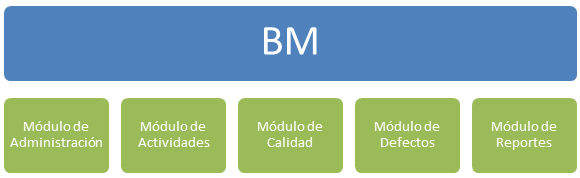
\includegraphics[scale=0.9]{images/ModulosBM.png}
	\caption{M'odulos del BM}
	\label{fig:ModulosBM}
\end{figure}

\subsection{Tipos de Usuario}
\noindent
El BM tendr'a tres tipos de usuarios: Administrador, L'ider de Proyecto y Usuario.  Est'an representados en la figura \ref{fig:UsuariosBM} que nos muestra los usuarios por nivel. Se representa en una pir'amide invertida para denotar los privilegios y que los niveles superiores tienen toda la funcionalidad de los niveles inferiores. Entonces el Administrador puede utilizar la funcionalidad del L'ider de Proyecto y del Usuario; mientras que el L'ider de Proyecto tiene acceso a la funcionalidad de Usuario.

\begin{figure}[h]
	\centering
		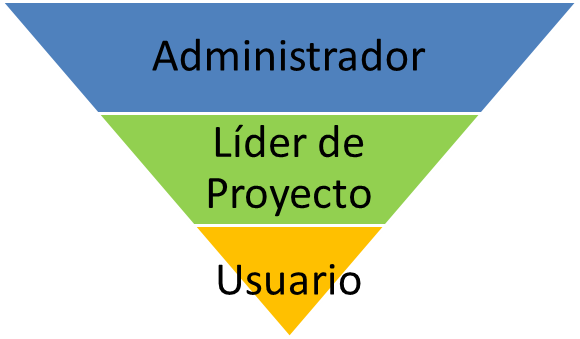
\includegraphics[scale=0.7]{images/UsuariosBM.png}
	\caption{Tipos de usuario del BM}
	\label{fig:UsuariosBM}
\end{figure}

Sus caracter'isticas y funcionalidades principales son: 

\begin{itemize}
	\item \emph{Administrador}. Es el tipo de usuario con m'as privilegios en el sistema y tiene responsabilidades y derechos a nivel organizaci'on, representa a la gerencia de la organizaci'on. Sus actividades principales son:
	\begin{itemize}
		\item Alta, baja y modificaci'on de proyectos.
		\item Alta, baja y modificaci'on de usuarios.
		\item Asignaci'on de recursos a proyectos.
		\item Revisi'on de reportes y m'etricas por organizaci'on, proyecto e individuales.
	\end{itemize}
	\item \emph{L'ider de Proyecto}. Es el tipo de usuario que le sigue en privilegios al Administrador y tiene responsabilidades y derechos a nivel de proyecto, representa al l'ider de uno o varios proyectos. Sus actividades principales son:
	\begin{itemize}
		\item Definici'on de tipos de defecto.
		\item Definici'on de ciclo de vida para el proyecto.
		\item Definici'on de plantillas p'ublicas para las actividades de calidad.
		\item Definici'on de actividades de desarrollo y de actividades de calidad.
		\item Asignaci'on de las actividades a los usuarios.
		\item Revisi'on de reportes y m'etricas a nivel proyecto e individuales.
	\end{itemize}
	\item \emph{Usuario}. Es el tipo de usuario con menos privilegios, representa un desarrollador del proyecto. Sus actividades principales son:	
	\begin{itemize}
		\item Seguimiento de las actividades asignadas.
		\item Creaci'on y modificaci'on de plantillas de calidad propias.
		\item Reporte de defectos.
		\item Seguimiento de defectos asignados.
		\item Revisi'on de reportes y m'etricas individuales.
	\end{itemize}
\end{itemize}

Los detalles de las funcionalidades completas del sistema ser'an descritas en la secci'on \ref{sec:funcionalidadesdelbm}.

\subsection{Impacto}
\label{sec:impacto}
\noindent
El BM impacta a los distintos niveles de cualquier organizaci'on dedicada al desarrollo de software.

\begin{itemize}
	\item A nivel de alta gerencia:
	\begin{itemize}
		\item Provocar'a una mayor formalidad en la manera de controlar y asignar recursos a nuevos y existentes proyectos.
		\item Dar'a una visibilidad del costo de la calidad que tienen los distintos proyectos de software.
		\item Permitir'a conocer el esfuerzo real que toman los proyectos y hacer compromisos con m'as informaci'on en el futuro.
	\end{itemize}
	\item A nivel de l'ider de proyecto:
		\item Dar'a una mayor formalidad y disciplina para la realizaci'on de actividades de planeaci'on referentes al ciclo de vida y a la calidad del producto. 
		\item Brindar'a una mejor visibilidad del estado actual del proyecto.
		\item Ayudar'a a realizar una administraci'on racional del proyecto.
		\item Facilitar'a la administraci'on de la calidad del proyecto.
	\item A nivel de desarrollador se tiene el mayor impacto:	
	\begin{itemize}
		\item Implicar'a que los desarrolladores cuenten con la suficiente disciplina para realizar las actividades de calidad de la mejor manera posible.
		\item Al registrar los defectos cometidos crear'a conciencia de estos dando un impacto inmediato a la calidad.
		\item Ayudar'a a los desarrolladores a mejorar sus procesos personales de desarrollo.
		\item Se generar'an estad'isticas y m'etricas con informaci'on ver'idica la cual permitir'a analizar los procesos y mejorar las 'areas m'as d'ebiles.
		\item En resumen, mejorar'a la forma en que los desarrolladores hacen su trabajo, haciendo que los productos que elaboren tengan una mayor calidad desde el inicio recortando el costo y el calendario de los proyectos.
	\end{itemize}
\end{itemize}

\subsection{Limitaciones}
\noindent
Dentro de las limitaciones identificadas para el sistema BM se encuentran:

\begin{itemize}
	\item Si bien se permite el acceso a m'ultiples usuarios de manera simult'anea, la concurrencia al momento de edici'on no est'a permitida.
	\item La generaci'on de estad'isticas y m'etricas se basa en la informaci'on y los datos introducidos por los distintos usuarios, por lo que en caso de que esta informaci'on no sea adecuada, las estad'isticas y m'etricas generadas por el sistema tampoco lo ser'an.
	\item El acceso al sistema depende de la correcta operaci'on de la red local de la empresa o del proveedor de servicios de Internet.
	\item La asignaci'on de restricciones y privilegios sobre el uso de la aplicaci'on para los diferentes tipos de usuarios est'a preestablecida, por lo que el cliente no podr'a configurar estos permisos al momento de la instalaci'on del sistema.
	\item Las estad'isticas y m'etricas generadas por el sistema fueron determinadas con anterioridad, por lo que el cliente no tendr'a la posibilidad de agregar, modificar o eliminar estad'isticas o m'etricas.
\end{itemize}

\section{Dise'no del Sistema}
\noindent
El BM est'a construido con las siguientes tecnolog'ias:

\begin{itemize}
	\item Java 7 EE como lenguaje de prop'osito general.
	\item Spring como infraestructura para crear la aplicaci'on web.
	\item MySQL como administrador de la base de datos.
	\item Velocity para realizar el scripting de las p'aginas web.
	\item Jquery para enriquecer la funcionalidad de las p'aginas web.
\end{itemize}

Con la combinaci'on y uso de las tecnolog'ias mencionadas se cre'o el BM. La arquitectura del sistema y el dise'no de la base de datos ser'an presentadas en las secciones consecuentes.

\subsection{Arquitectura}
\noindent
La arquitectura del BM se muestra en la figura \ref{fig:ArquitecturaBM}. Los componentes de esta son los siguientes:

\begin{itemize}
	\item \emph{Vista}. En esta capa se encuentran los archivos que visualiza el usuario final. Estos archivos est'an construidos en c'odigo HTML din'amicamente por Velocity y son enriquecidos con Jquery.
	\item \emph{Controladores}. Es la capa de conexi'on entre la Vista y la Capa de Negocios. Est'a encargada de recibir las solicitudes de la Vista, llamar a la Capa de Negocios para realizar las operaciones y mandar los resultados de nuevo a la Vista.
	\item \emph{Capa de Negocios}. Es la capa de conexi'on entre los Controladores y el Modelo. En esta capa est'a implementada la funcionalidad del sistema y contiene las operaciones por realizarse.
	\item \emph{Modelo}. Es la capa de conexi'on entre la Capa de Negocios y del DAO. Esta capa es una representaci'on de la base de datos. Es utilizada por la Capa de Negocios para crear los objetos, y obtiene los datos de estos objetos a trav'es del DAO.
	\item \emph{DAO}. El objeto de acceso a la base de datos (por sus siglas en Ingl'es DAO) es la capa que conecta la base de datos con el modelo. Esta capa se encarga de recibir solicitudes de informaci'on por parte del Modelo, obtiene la informaci'on de la base de datos y la regresa al modelo.
	\item \emph{Base de Datos}. Es el contenedor que almacena la informaci'on de todo el BM.
\end{itemize}

\begin{figure}[h]
	\centering
		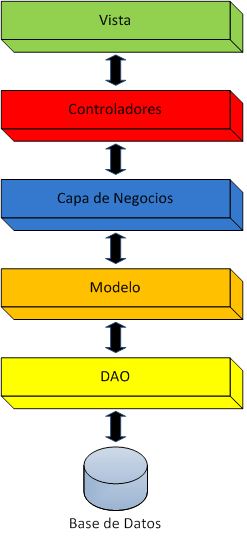
\includegraphics[scale=0.8]{images/ArquitecturaBM.png}
	\caption{Arquitectura del BM}
	\label{fig:ArquitecturaBM}
\end{figure}

\subsection{Base de Datos}
\noindent
La figura \ref{fig:dbBM} nos muestra el dise'no de la base de datos. 

\begin{figure}[h]
	\centering
		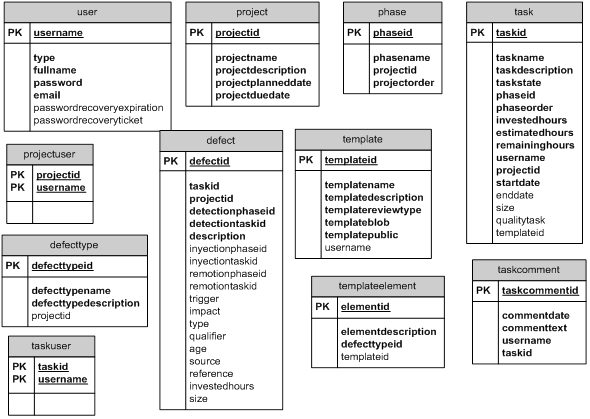
\includegraphics[scale=0.95]{images/dbBM.png}
	\caption{Base de Datos del BM}
	\label{fig:dbBM}
\end{figure}

Esta contiene las siguientes tablas:

\begin{itemize}
	\item \emph{User}. Contiene los usuarios del sistema.
	\item \emph{Project}. Contiene los proyectos del sistema.
	\item \emph{Phase}. Contiene las fases del sistema. Cada fase pertenece a un proyecto en espec'ifico.
	\item \emph{Task}. Contiene las tareas del sistema. Cada tarea est'a relacionada con un proyecto y con una fase del proyecto y puede ser una tarea de desarrollo o de calidad.
	\item \emph{Taskcomment}. Contiene los comentarios realizados en las tareas. Se relaciona con una tarea.
	\item \emph{Defect}. Contiene los defectos registrados en el sistema. Los defectos est'an relacionados con la tarea y la fase en la que fueron detectados.
	\item \emph{Template}. Contiene las plantillas que sirven como gu'ias para las actividades de calidad del sistema. Estas plantillas pueden ser p'ublicas o privadas. Inicia con la plantilla para lenguajes de prop'osito general propuesta por Humphrey\cite{Humphrey}.
	\item \emph{Templateelement}. Representa un elemento dentro de las plantillas de calidad, est'a relacionado a una plantilla en espec'ifico.
	\item \emph{Defecttype}. Contiene los tipos de defectos del sistema. Inicia con los tipos de defectos del PSP\cite{Humphrey}.
	\item \emph{Projectuser}. Es una tabla de soporte que ayuda a relacionar varios proyectos con varios usuarios.
	\item \emph{Taskuser}. Es una tabla de soporte que ayuda a relacionar varios usuarios con varias tareas.
\end{itemize}

\section{Funcionalidades del BM}
\label{sec:funcionalidadesdelbm}
\noindent
En esta secci'on se describir'an a detalle las secciones del BM. Encontraremos dos tipos de funcionalidades:

\begin{itemize}
	\item \emph{Funcionalidades de Administraci'on}. Estas funciones son aquellas necesarias para el correcto funcionamiento del sistema, como puede ser administraci'on de usuarios y de proyectos.
	\item \emph{Funcionalidades de Valor Agregado}. Estas funciones son aquellas que ayudan a las empresas a obtener los beneficios mencionados en la secci'on~\ref{sec:impacto}. En estas se har'a referencia a los objetivos que tienen y como son soportadas por la teor'ia.
\end{itemize}

\subsection{Administraci'on de Usuarios}
\noindent
Esta parte del sistema es meramente administrativa y solo los usuarios . Tiene las siguientes funcionalidades:

\begin{itemize}
	\item \emph{Alta de Usuarios}. Se registran nuevos usuarios especificando su nombre de usuario, nombre real, correo electr'onico, privilegios y contrase'na.
	\item \emph{Modificaci'on de Usuarios}. Se pueden editar los campos dados de alta en el Alta excepto la contrase'na.
	\item \emph{Cambio de Contrase'na}. Existe una pantalla especial para el cambio de contrase'na y recuperaci'on de esta en caso de haberla perdido.
	\item \emph{Eliminaci'on de Usuarios}. Se pueden eliminar los usuarios siempre y cuando no sea el usuario ``admin'' (usuario por default del sistema) y no est'e enrolado en ning'un proyecto.
\end{itemize}

\subsection{Administraci'on de Recursos}
\noindent
Otra parte del sistema administrativa pero con su grado de importancia. En esta secci�n un usuario con privilegios de administrador puede asignar a los diferentes usuarios del sistema a los proyectos existentes. Un usuario al ser asignado a un proyecto obtiene autom�ticamente la visibilidad de este.

\subsection{Administraci'on de Proyectos}
\noindent
Esta parte del sistema permite al administrador las siguientes funcionalidades:

\begin{itemize}
	\item \emph{Alta de Proyectos}. Se dan de alta nuevos proyectos especificando nombre del proyecto, descripci'on breve, fecha de entrega planeada y fecha de entrega real. Despu'es de dar de alta un proyecto se pasa a la creaci'on de su ciclo de vida.
	\item \emph{Modificaci'on de Proyectos}. Se pueden modificar los datos de los proyectos registrados en su alta. Aparte se especifica la fase actual en la que se encuentra el proyecto.
	\item \emph{Eliminaci'on de Proyectos}. Los proyectos pueden ser eliminados solamente cuando no tengan informaci'on registrada dentro de estos.
\end{itemize}

\subsection{Ciclo de Vida de Proyectos}
\label{sec:ciclodevidadeproyectos}
\noindent
El BM permite al administrador o al l'ider de proyecto la creaci'on de un ciclo de vida propio para el proyecto, o la selecci'on de uno predefinido que puede ser:

\begin{itemize}
	\item \emph{Cascada}. Es el ciclo de vida m'as cl'asico de los proyectos de desarrollo de software. Tiene las fases de Requerimientos, Dise'no, Codificaci'on, Pruebas y Mantenimiento.
	\item \emph{Iterativo}. Es el ciclo de vida preferido por los proyectos desarrollados en empresas con filosof'ias 'agiles. Este ciclo es una variaci'on del ciclo de vida de cascada, pero en vez de realizar el dise'no, la codificaci'on y las pruebas completas en una sola ocasi'on, dividen estas tres tareas en varias iteraciones para enfrentar los posibles cambios.
\end{itemize}

La figura \ref{fig:SSciclo1BM} nos muestra la pantalla donde se permite elegir los ciclos de vida. Una vez seleccionado un ciclo de vida default o comenzando a crear uno propio se pueden agregar, modificar o eliminar las fases existentes como se muestra en la figura \ref{fig:SSciclo2BM}. Una fase no puede ser eliminada una vez que tenga actividades registradas. Los datos que contiene una fase de un proyecto son: Nombre, tipo, descripci'on y orden en el proyecto.

Los tipos de fase predefinidos en el BM son los siguientes:

\begin{itemize}
	\item \emph{Requerimientos}. Esta es la fase donde se realiza la licitaci'on y el an'alisis de los requerimientos del proyecto.
	\item \emph{Dise'no}. En esta fase se toman las decisiones m'as importantes respecto a como ser'a construido el proyecto. Lo que se realice en esta fase determinar'a como es que el proyecto funcionar'a y si tendr'a 'exito o no. Los productos de trabajo de esta fase m'as comunes son la arquitectura y el dise'no detallado.
	\item \emph{Codificaci'on}. En esta fase se construye el sistema, tambi'en es llamada fase de construcci'on o programaci'on. Es la etapa de programaci'on y la primera que nos viene a la mente en el desarrollo de software.
	\item \emph{Revisi'on}. Esta fase puede ser utilizada como comod'in. Se incluy'o en caso de que el equipo de desarrollo decida agregar alguna fase completa de revisi'on de los productos de otra fase. Ya que el costo de los errores aumenta exponencialmente conforme avanza de fases el proyecto\cite{Lazic2009}, entonces es muy importante evitar la inyecci'on de errores en fases tempranas como Requerimientos y Dise'no, as'i que podr'ia incluirse una fase completa para realizar actividades como inspecciones al dise'no y a los requerimientos. En caso de que se decida no utilizar una fase completa para revisiones, es muy importante que al menos se realicen revisiones personales al trabajo realizado.
	\item \emph{Pruebas}. Esta etapa corresponde a las pruebas cl'asicas. Se recomienda al menos la realizaci'on de pruebas unitarias y de sistema.
	\item \emph{Mantenimiento}. Esta fase es cuando el sistema ha salido a producci'on y se contin'uan agregando nuevas funcionalidades o defectos encontrados por el cliente. El objetivo del BM es que no haya ning'un defecto reportando por el cliente.
\end{itemize}

\begin{figure}[h]
	\centering
		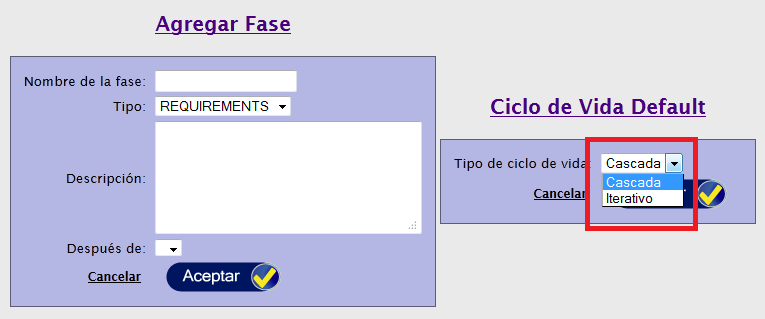
\includegraphics[scale=0.8]{images/SSciclo1BM.png}
	\caption{Ciclo de Vida Default}
	\label{fig:SSciclo1BM}
\end{figure}

\begin{figure}[h]
	\centering
		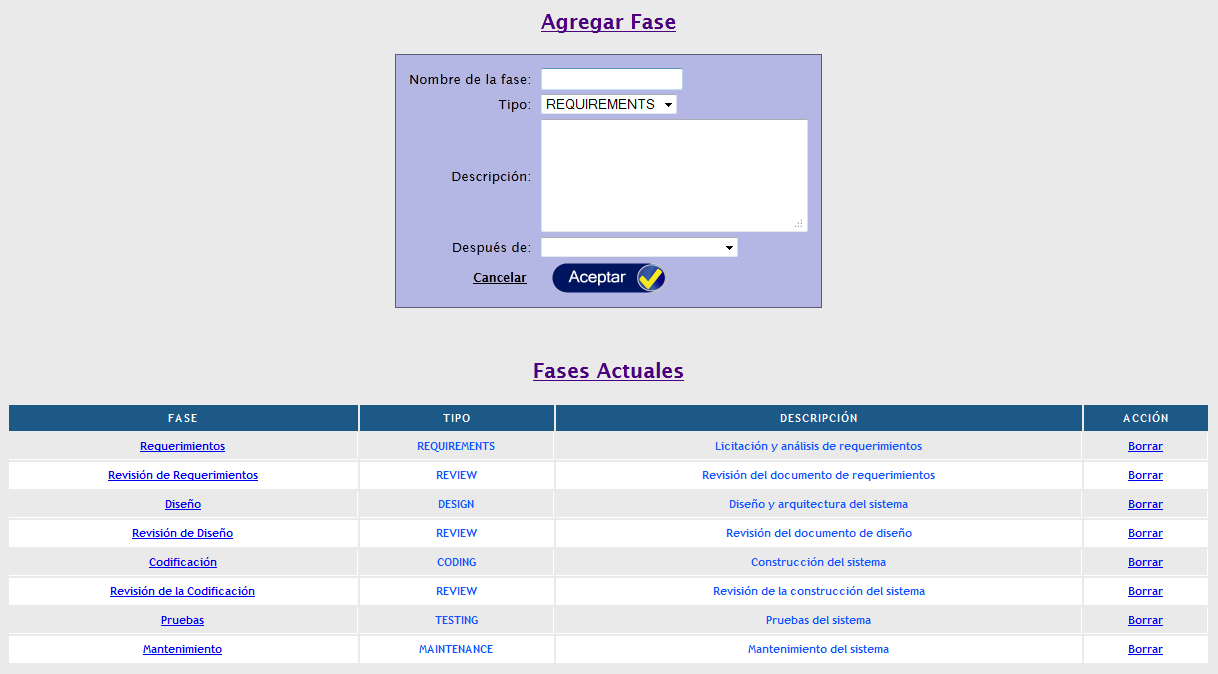
\includegraphics[scale=0.5]{images/SSciclo2BM.png}
	\caption{Edici'on del Ciclo de Vida}
	\label{fig:SSciclo2BM}
\end{figure}

Es importante destacar que la definici'on del ciclo de vida es el primer paso para iniciar la planeaci'on del proyecto. La planeaci'on es una de las pr'acticas recomendadas por \cite{Humphrey2002} para realizar la administraci'on racional. Si una organizaci'on quiere tener 'exito en el negocio del software es clave la planeaci'on del proyecto.

Para el uso correcto del BM y obtener su mayor potencial se recomienda una definici'on a conciencia del ciclo de vida. Una vez definido el ciclo de vida se puede pasar a la definici'on de las tareas dentro de cada fase. Tambi'en es de suma importancia que cada una de estas tareas cuente con su actividad de revisi'on, para fomentar la cultura de la prevenci'on antes de las pruebas.

\subsection{Administraci'on  y Seguimiento de Actividades}
\label{sec:administracionyseguimientodeactividades}
\noindent
El registro, actualizaci'on y medici'on de las actividades realizadas dentro de un proyecto es clave para hacer un trabajo de calidad. Lo que es medido es administrado, y lo que es administrado se hace correctamente, en cambio, lo que no es medido no se administra y por lo tanto no se termina\cite{Humphrey2002}. 

El BM facilita la labor de la planeaci'on y administraci'on de actividades por medio de distintas funcionalidades:

\begin{itemize}
	\item La creaci'on de un ciclo de vida para el proyecto como se explic'o en la secci'on \ref{sec:ciclodevidadeproyectos}.
	\item El alta, baja y modificaci'on de actividades.
	\item El seguimiento y actualizaci'on de las actividades.
\end{itemize}

El BM tiene dos tipos de actividades:

\begin{itemize}
	\item \emph{Actividades de Desarrollo}. En esta categor'ia caen todas las actividades relacionadas con el proceso de desarrollo de software en las cuales se generan productos de trabajo. Ejemplos de estas son: Licitaci'on de requerimientos, dise'no detallado del m'odulo de un sistema, programaci'on, pruebas unitarias entre otras. Este tipo de actividades tienen subtipos, estos son los siguientes:	
	\begin{itemize}
		\item \emph{REQUIREMENTS}. Actividades relacionadas a una fase de requerimientos.
		\item \emph{DESIGN}. Actividades relacionadas a una fase de dise'no.
		\item \emph{DEVELOPMENT}. Actividades relacionadas a la fase de construcci'on.
		\item \emph{TESTING}. Actividades relacionadas con alguno de los tipos de prueba mencionados en la secci'on \ref{sec:pruebasdesoftware}.
	\end{itemize}
\end{itemize}

\begin{itemize}
	\item \emph{Actividades de Calidad}. Son las actividades de prevenci'on y evaluaci'on realizadas en el proyecto de desarrollo las cuales nos ayudan a evitar la inyecci'on de defectos o a detectarlos lo antes posible dentro del ciclo de desarrollo. Las actividades de calidad que maneja el BM, las cuales fueron descritas a detalle en la secci'on \ref{sec:tecnicasdedetecciondedefectos}, son las siguientes:
	\begin{itemize}
		\item \emph{PERSONAL REVIEW}. Actividades donde se realiza una revisi'on personal a un producto de trabajo.
		\item \emph{PEER REVIEW}. Actividades donde se realiza una revisi'on entre colegas de un producto de trabajo.
		\item \emph{WALKTHROUGH}. Actividades donde se realiza una caminata a un producto de trabajo.
		\item \emph{INSPECTION}. Actividades donde se realiza una inspecci'on a un producto de trabajo.
	\end{itemize}
\end{itemize}

Para obtener mayores beneficios del BM y tener un nivel 'optimo de calidad se recomienda la siguiente forma de trabajo:

\begin{itemize}
	\item Realizar al menos una revisi'on personal a cada producto de trabajo utilizando una plantilla de calidad. Por ejemplo cada que el desarrollador termine de programar un clase del sistema, realizar una revisi'on personal de esta apoy'andose con la plantilla de calidad default o una elaborada personalmente.
	\item Realizar una inspecci'on a cada producto mayor de trabajo. Un producto mayor de trabajo es un producto que representa el cierre de una fase, por ejemplo: El documento de requerimientos al terminar la fase de requerimientos, la arquitectura del sistema al terminar el dise'no conceptual, entre otros.	
\end{itemize}

Las funcionalidades b'asicas con las actividades tanto de desarrollo como de calidad son las siguientes:

\begin{itemize}
	\item \emph{Alta de actividades}. Se registra una nueva actividad en el sistema con los siguientes datos: Nombre de la tarea, tipo, fase, descripci'on, esfuerzo planeado, reponsable, fecha de inicio y fecha meta. La forma se puede ver en la figura \ref{fig:SSagregartareaBM}.
	\item \emph{Modificaci'on de actividades}. Se modifican los datos con los cuales se dieron de alta las actividades.
	\item \emph{Baja de actividades}. Una actividad puede ser dada de baja solo en el caso de que no tenga registrado esfuerzo.
\end{itemize}

\begin{figure}[h]
	\centering
		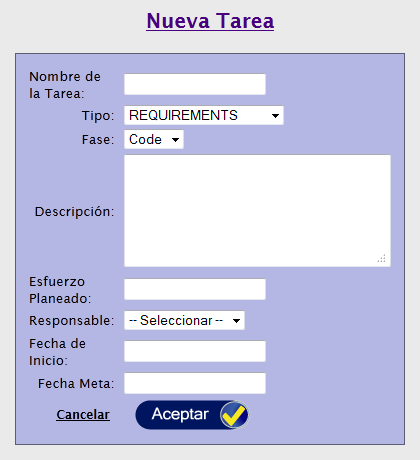
\includegraphics[scale=0.9]{images/SSagregartareaBM.png}
	\caption{Creaci'on de Actividades}
	\label{fig:SSagregartareaBM}
\end{figure}

El seguimiento de las actividades se muestra en la figura \ref{fig:SSseguirtarea1BM}. Esto nos permitir'a hacer un seguimiento y administraci'on adecuado de cada tarea. Se recomienda que diariamente el responsable de la actividad haga una actualizaci'on de esta con las siguientes consideraciones:

\begin{itemize}
	\item Escribir en el campo de Agregar Esfuerzo el n'umero de horas reales que le dedic'o a la tarea. Por ejemplo: Un desarrollador tiene como tarea programar la interfaz de un sistema un d'ia de trabajo; pero en el d'ia de 8 horas, pas'o 2 horas en juntas, otra hora revisando el correo electr'onico y una hora m'as en descansos, entonces ese d'ia debe reportar 4 horas al esfuerzo y no las 8 horas del d'ia. Esto es muy importante para que las empresas identifiquen las horas reales de trabajo que tienen los desarrolladores y as'i puedan hacer m'as eficiente el tiempo en la oficina.
	\item Si el esfuerzo restante se deja en 0 la actividad ser'a marcada como terminada, as'i que es importante que se estime el esfuerzo restante y se coloque en el campo respectivo. Esto ayudar'a a los desarrolladores a mejorar sus habilidades de estimaci'on y generar datos hist'oricos.
	\item Colocar el tama'no de la tarea en las unidades que maneje la empresa. Para el uso del BM se recomienda utilizar LOC para los programas por su facilidad al momento de calcular y lo com'un que es dentro de la industria, sin embargo se pueden utilizar otras m'etricas como puntos de funci'on. Esto tambi'en ayudar'a a crear datos hist'oricos y facilitar'a el dimensionamiento de futuros proyectos.
	\item Agregar comentarios para cada suceso importante que surja en las actividades. Los comentarios quedar'an registrados y ser consultados despu'es.
	\item Tener en cuenta que la Fecha Fin no es la fecha en que se finaliz'o la tarea, si no la fecha en que estaba planeado en que se finalizara. La fecha cuando se finaliza la tarea se registra de forma autom'atica cuando el estatus de la tarea pasa a COMPLETADA. 
\end{itemize}

\begin{figure}[h]
	\centering
		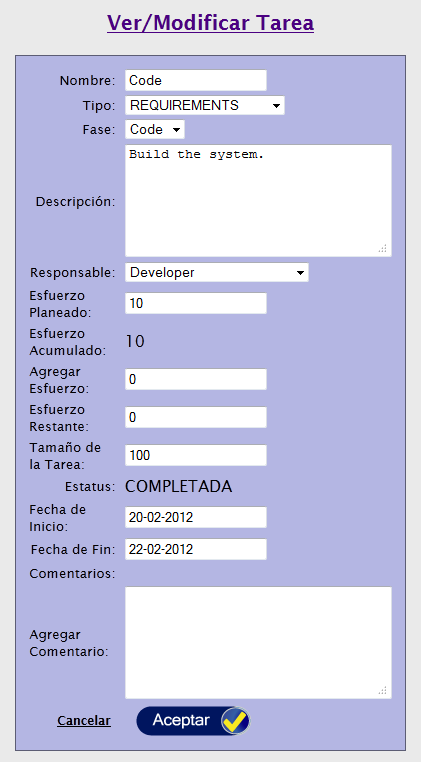
\includegraphics[scale=0.7]{images/SSseguirtarea1BM.png}
	\caption{Seguimiento de Actividades}
	\label{fig:SSseguirtarea1BM}
\end{figure}

\subsection{Administraci'on  y Seguimiento de Defectos}
\label{sec:administracionyseguimientodedefectos}
\noindent

\clearpage